\section{Reconstructing synthetic distributions} \label{sec:synthetic_distributions}

Before applying the optimal transport methodology to orbital mechanics, it is necessary to isolate and evaluate the representational capacity of the KR map. Testing the framework on synthetic distributions provides a simple and immediate empirical validation, independent of the confounding variables introduced by physical propagation models. By evaluating the methodology on artificial, non-linear geometries, the capacity to capture non-trivial structural deformations can be assessed without relying on external dynamics. Thus, this phase focuses purely on the geometric limits of the mapping procedure.

To generate the synthetic test cases, a known structural deformation is applied to a reference probability measure. The target distribution is represented by a finite set of $n$ unmapped particles, denoted as $\{x^{(i)}\}_{i=1}^n \subset \mathbb{R}^D$, where $D$ denotes the physical state dimension. These particles are generated by applying a non-linear artificial shear mapping, $\tilde{S}: \mathbb{R}^D \to \mathbb{R}^D$, to full state samples drawn from a multivariate standard normal distribution, $\{\tilde{z}^{(i)}\}_{i=1}^n$, where $\tilde{z}^{(i)} \sim \mathcal{N}(0, I_D)$. The shear mapping takes the form
\begin{equation*}
    x^{(i)} = \tilde{S} \left( \tilde{z}^{(i)} \right), \quad i = 1, \dots, n.
\end{equation*}

The reconstruction objective is to approximate the inverse transformation, mapping $S : \mathbb{R}^D \to \mathbb{R}^D$, that transports the sheared particles $\{x^{(i)}\}_{i=1}^n$ back to standard normal distribution. This produces a new set of mapped particles $\{z^{(i)}\}_{i=1}^n$. The success of the reconstruction is evaluated by comparing the empirical distribution of $\{z^{(i)}\}_{i=1}^n$ against the original unsheared particles $\{\tilde{z}^{(i)}\}$, thereby quantifying the ability of the algorithm to invert the artificial shear $\tilde{S}$.

\subsection{Numerical results} \label{subsec:synthetic_results}

The framework is tested against three distinct synthetic shear models. For these experiments, the state dimension is restricted to $D = 2$, which is chosen for ease of visualisation. We denote the spatial components of the true normal samples as $\tilde{z}^{(i)} = (\tilde{z}^{(i)}_1, \tilde{z}^{(i)}_2)^T$ and the resulting sheared target particles as $x^{(i)} = (x^{(i)}_1, x^{(i)}_2)^T$.

The first test case introduces a linear shear that pushes the particles on a straight line, applying an off-diagonal structural deformation to the state space. The transformation takes the form
\begin{align*}
    x^{(i)}_1 &= \tilde{z}^{(i)}_1 - 0.85 \tilde{z}^{(i)}_2, \\
    x^{(i)}_2 &= \tilde{z}^{(i)}_2.
\end{align*}
This shear provides a baseline for testing the framework's capability to invert highly correlated, off-diagonal linear deformations.

The second test case involves a quadratic shear. The mapping is defined as
\begin{align*}
    x^{(i)}_1 &= \tilde{z}^{(i)}_1, \\
    x^{(i)}_2 &= \tilde{z}^{(i)}_2 + \left( \tilde{z}^{(i)}_1 \right)^2.
\end{align*}
This quadratic warping is a prevalent characteristic of orbital uncertainty propagation over short to medium time horizons, making this synthetic case a rough approximation to the physical aerospace application. This acts as a first-order test to ensure feasibility on the full orbital uncertainty experiment, which we will later discuss in Section~\ref{sec:aerospace_uncertainty}. \newpage

The final synthetic experiment employs a cubic shear. The transformation is given by
\begin{align*}
    x^{(i)}_1 &= \tilde{z}^{(i)}_1, \\
    x^{(i)}_2 &= \tilde{z}^{(i)}_2 + 0.4 \left( \left( \tilde{z}^{(i)}_1 \right)^3 - \tilde{z}^{(i)}_1 \right).
\end{align*}
The cubic shear subjects the baseline probability measure to higher-order polynomial deformations, requiring a higher-order polynomial expansion to be modelled, and therefore a higher number of map components to be optimised. This benchmark is therefore aimed at preliminarily testing the scaling capabilities of the optimal transport inexact projection framework.

The specific parameter configurations for each synthetic shear experiment are summarised in Table~\ref{tab:optimisation_parameters}. We remark that these parameters were chosen primarily through experience and guidance from literature works, the list of which would be hard to formulate and too long to recount. In addition, some parameter choices were refined through trial and error for each individual experience. We also note that several practical implementation details, such as additional numerical tolerances and specific architectural choices, are omitted from this discussion. This choice is aimed at preventing a verbose explanation of the numerics and keeping the reader focused on the more relevant implementation details.

\begin{table}[htbp]
    \centering
    \caption{Optimisation parameters used across the synthetic shear experiments.}
    \begin{tabular}{lcccc}
        \toprule
        \textbf{Parameter} & \textbf{Symbol} & \textbf{Linear} & \textbf{Quadratic} & \textbf{Cubic} \\
        \midrule
        Random seed & --                            & 2222 & 5432 & 507 \\
        State dimension & $D$                       & 2 & 2 & 2 \\
        Hermite degree & $J_k + 1$                  & 2 & 3 & 5 \\
        Particle count & $n$                        & 500 & 1000 & 500 \\
        Mini-batch cardinality & $B$                & 100 & 200 & 100 \\
        Outer PGD iterations & $T$                  & 10000 & 1000 & 5000 \\
        Dykstra budget & $M_{\mathrm{base}}$        & 10 & 10 & 10 \\
        Budget scaling exponent & $p$               & 0.5 & 0.67 & 0.54 \\
        Initial learning rate & $\eta^\circ$        & 0.2 & 0.1 & 0.01 \\
        Learning rate decay & $\gamma$              & 0.01 & 0.01 & 0.01 \\
        IHT interval & $K_{\mathrm{IHT}}$           & 100 & 100 & 100 \\
        IHT tolerance & $\varepsilon_p$             & 0.01 & 0.01 & 0.01 \\
        Monotonicity tolerance & $\varepsilon_m$    & 1e-12 & 1e-12 & 1e-12 \\
        
        \bottomrule
    \end{tabular}
    \label{tab:optimisation_parameters}
\end{table}

The sheared distributions, as well as final mapped results, are shown in Figure~\ref{fig:final_synthetic_distributions}.

\begin{figure}[htbp]
    \centering
    \begin{subfigure}[b]{\linewidth}
        \centering
        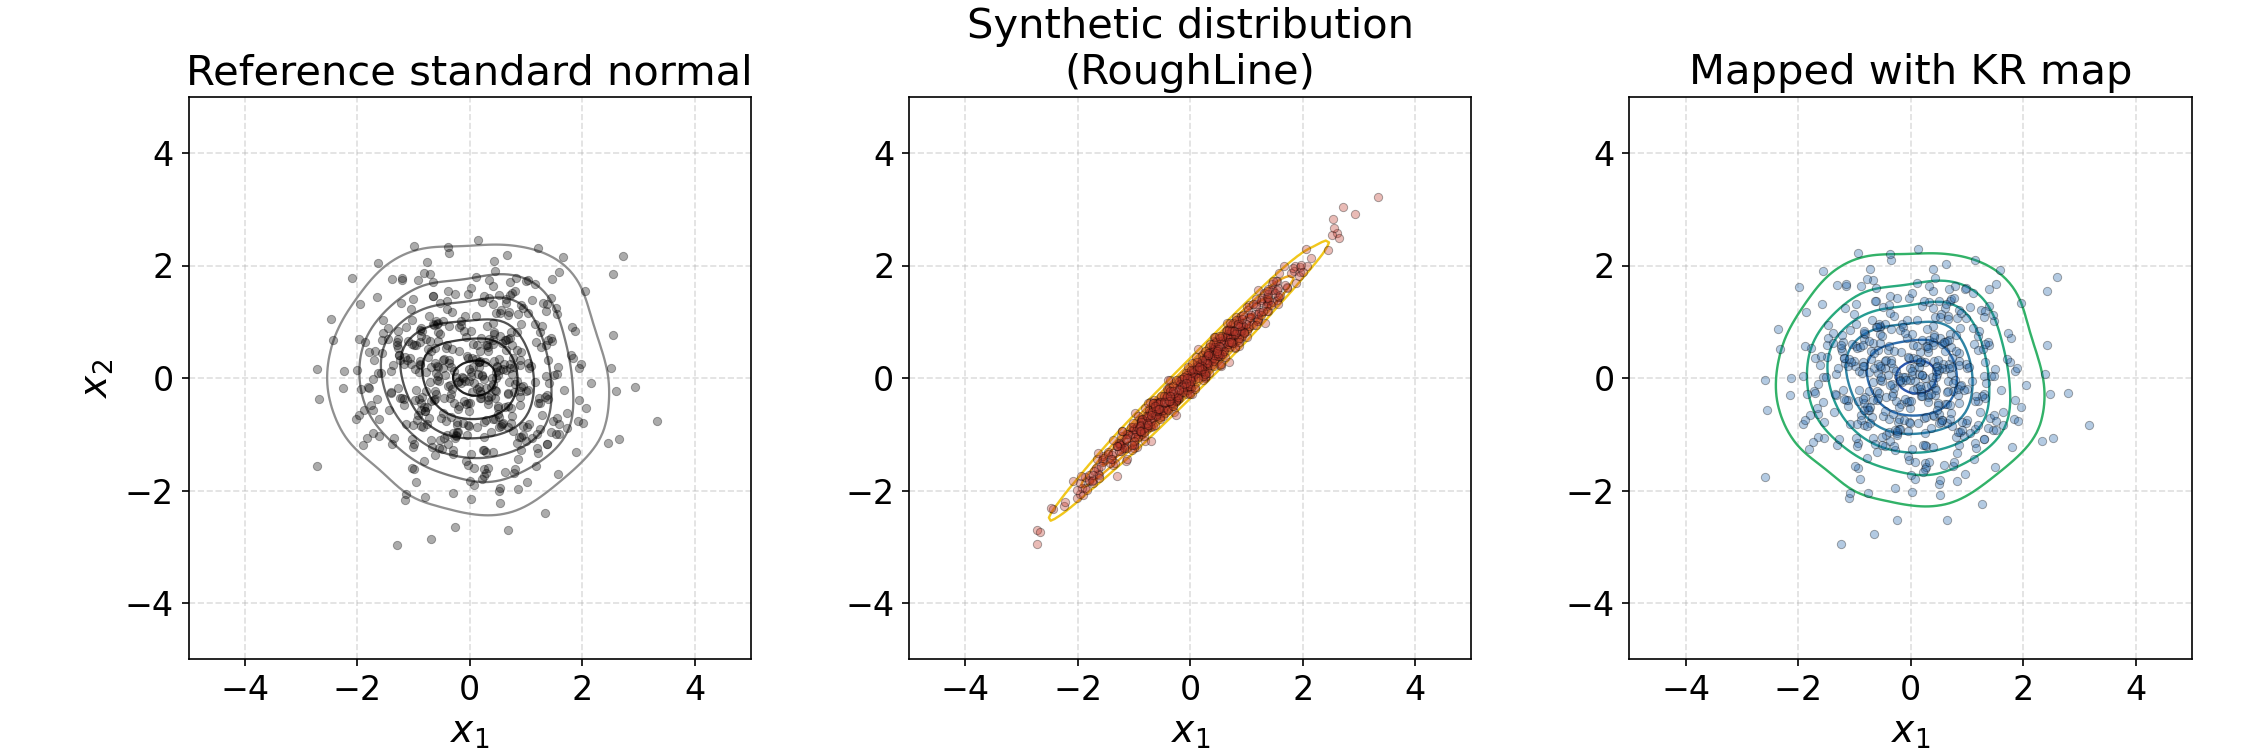
\includegraphics[width=\linewidth]{figures/line_shear_final.png}
        \caption{Results for the linear synthetic shear (\texttt{SEED} $=2222$).}
        \label{fig:line_shear_final}
    \end{subfigure}
    
    \vspace{1em}
    
    \begin{subfigure}[b]{\linewidth}
        \centering
        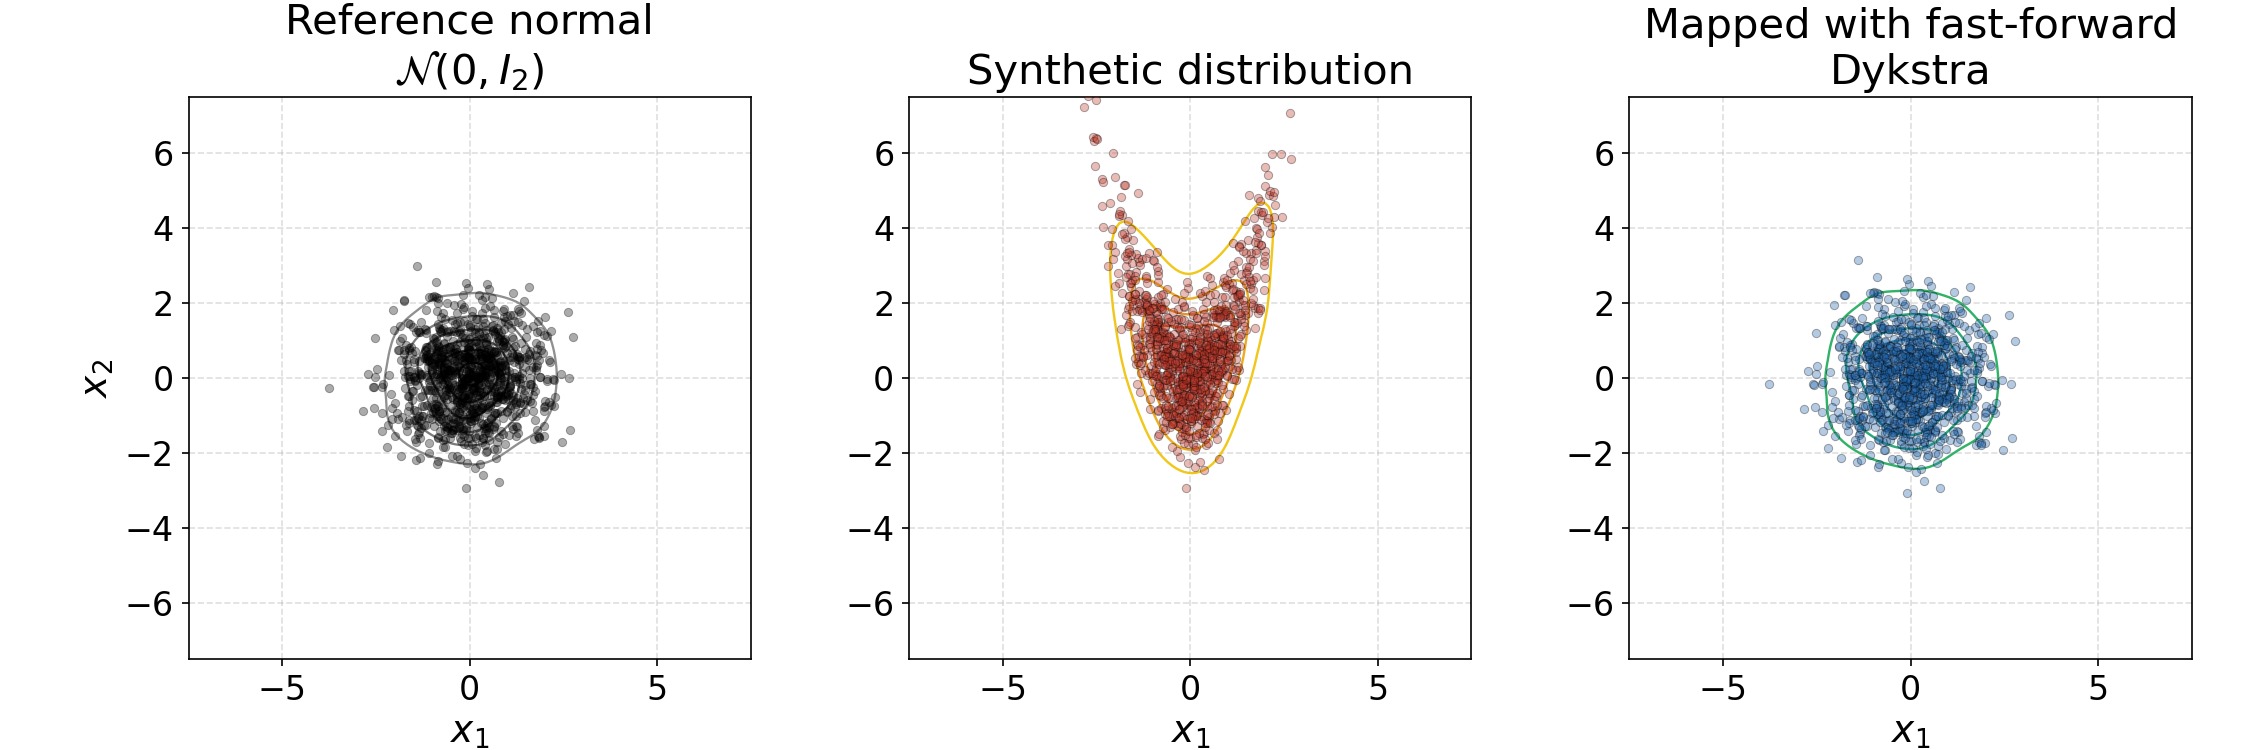
\includegraphics[width=\linewidth]{figures/quadratic_shear_final.png}
        \caption{Results for the quadratic synthetic shear (\texttt{SEED} $=5432$).}
        \label{fig:quadratic_shear_final}
    \end{subfigure}
    
    \vspace{1em}
    
    \begin{subfigure}[b]{\linewidth}
        \centering
        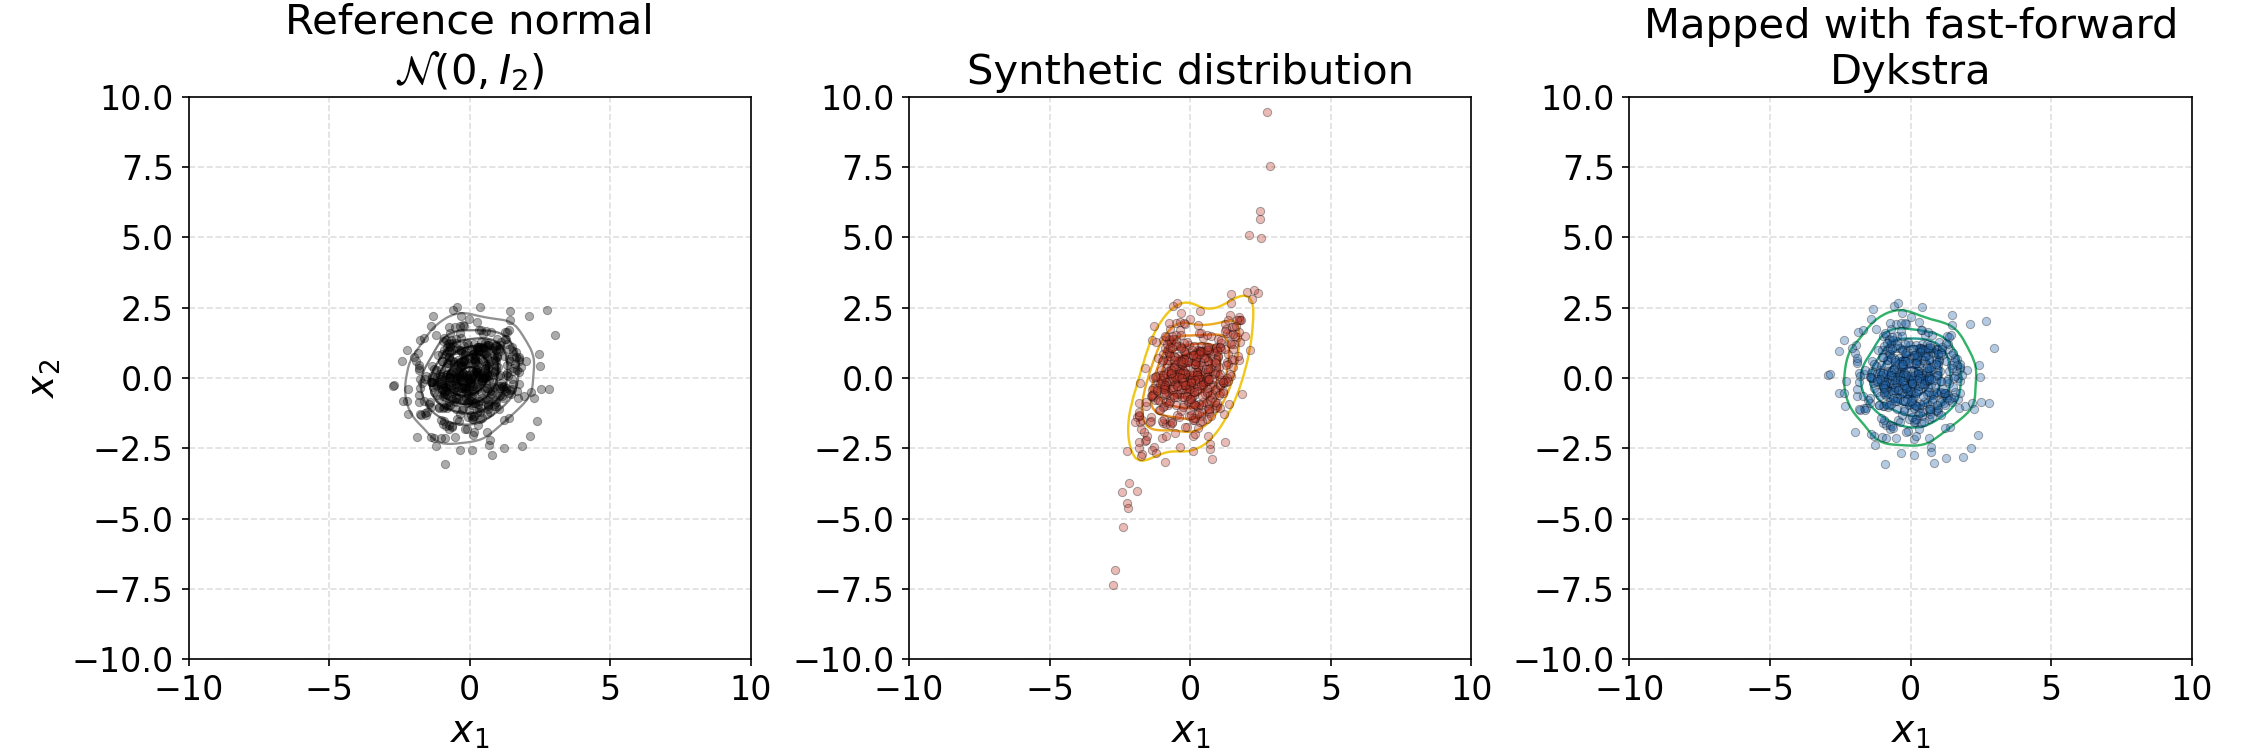
\includegraphics[width=\linewidth]{figures/cubic_shear_final.png}
        \caption{Results for the cubic synthetic shear (\texttt{SEED} $=507$).}
        \label{fig:cubic_shear_final}
    \end{subfigure}
    
    \caption{Reconstruction of the three synthetic shear distributions.}
    \label{fig:final_synthetic_distributions}
\end{figure}

The figure shows the linear, quadratic, and cubic models in Figures~\ref{fig:line_shear_final},~\ref{fig:quadratic_shear_final},~\ref{fig:cubic_shear_final}, respectively. The left-most panels show the unsheared particles $\{\tilde{z}^{(i)}\}$, the center panels the sheared particles $\{x^{(i)}\}$, and the right-most panels the mapped particles $\{z^{(i)}\}$. Distribution contours are also plotted for each panel\footnote{To visualise the geometric structure of the multidimensional states, iso-density contour lines are generated directly from the empirical particle sets rather than analytical probability density functions. The continuous density field is first approximated over a uniformly discretised spatial grid using either a Gaussian kernel density estimator or a smoothed two-dimensional spatial histogram. The resulting field is then discretised into a finite set of contour levels defined relative to the maximum evaluated density. By linearly spacing these isolines between $10\%$ and $95\%$ of the maximum density, the primary mass of the distribution is consistently captured while filtering low-density boundary artefacts.}.

Visual evaluation of the reconstructed distribution indicates that the mapped particles accurately reconstruct the reference state. To quantitatively substantiate this geometric recovery, the empirical Wasserstein-2 distance between the mapped empirical distribution and the theoretical standard normal measure was evaluated to below $10^{-2}$ across all three configurations.

To visualise the temporal evolution of the mapping procedure, the intermediate mapped states are evaluated at distinct intervals during the learning process. Progress plots, displaying the reconstructed distributions across varying outer projected gradient descent iterations, are presented in Figure~\ref{fig:line_shear_progress}, Figure~\ref{fig:quadratic_shear_progress}, and Figure~\ref{fig:cubic_shear_progress} for the linear, quadratic, and cubic models, respectively.

Table~\ref{tab:synthetic_runtimes} details the empirical execution time required to optimise the individual map components, $S^1$ and $S^2$, alongside the cumulative algorithmic runtime, for each synthetic distribution.

\begin{table}[htbp]
    \centering
    \caption{Runtime across the synthetic tests.}
    \label{tab:synthetic_runtimes}
    \begin{tabular}{@{}llccc@{}}
        & & \multicolumn{3}{c}{Runtime (s)} \\
        \cmidrule(l){3-5}
        Model & Seed & $S^1$ & $S^2$ & Total \\
        \midrule
        Linear & 2222 & 52.84 & 55.21 & 108.05 \\
        Quadratic & 5432 & 10.38 & 26.30 & 36.68 \\
        Cubic & 507 & 44.09 & 51.19 & 95.28 \\
        \bottomrule
    \end{tabular}
\end{table}

The quadratic deformation required the lowest total execution time. In contrast, the linear and cubic models demanded higher computational effort, yielding cumulative runtimes of 108.05 seconds and 95.28 seconds, respectively. Across all configurations, the optimisation of the two-dimensional component $S^2$ required greater computational duration than the one-dimensional component $S^1$, as expected.

\begin{figure}[htbp]
    \centering
    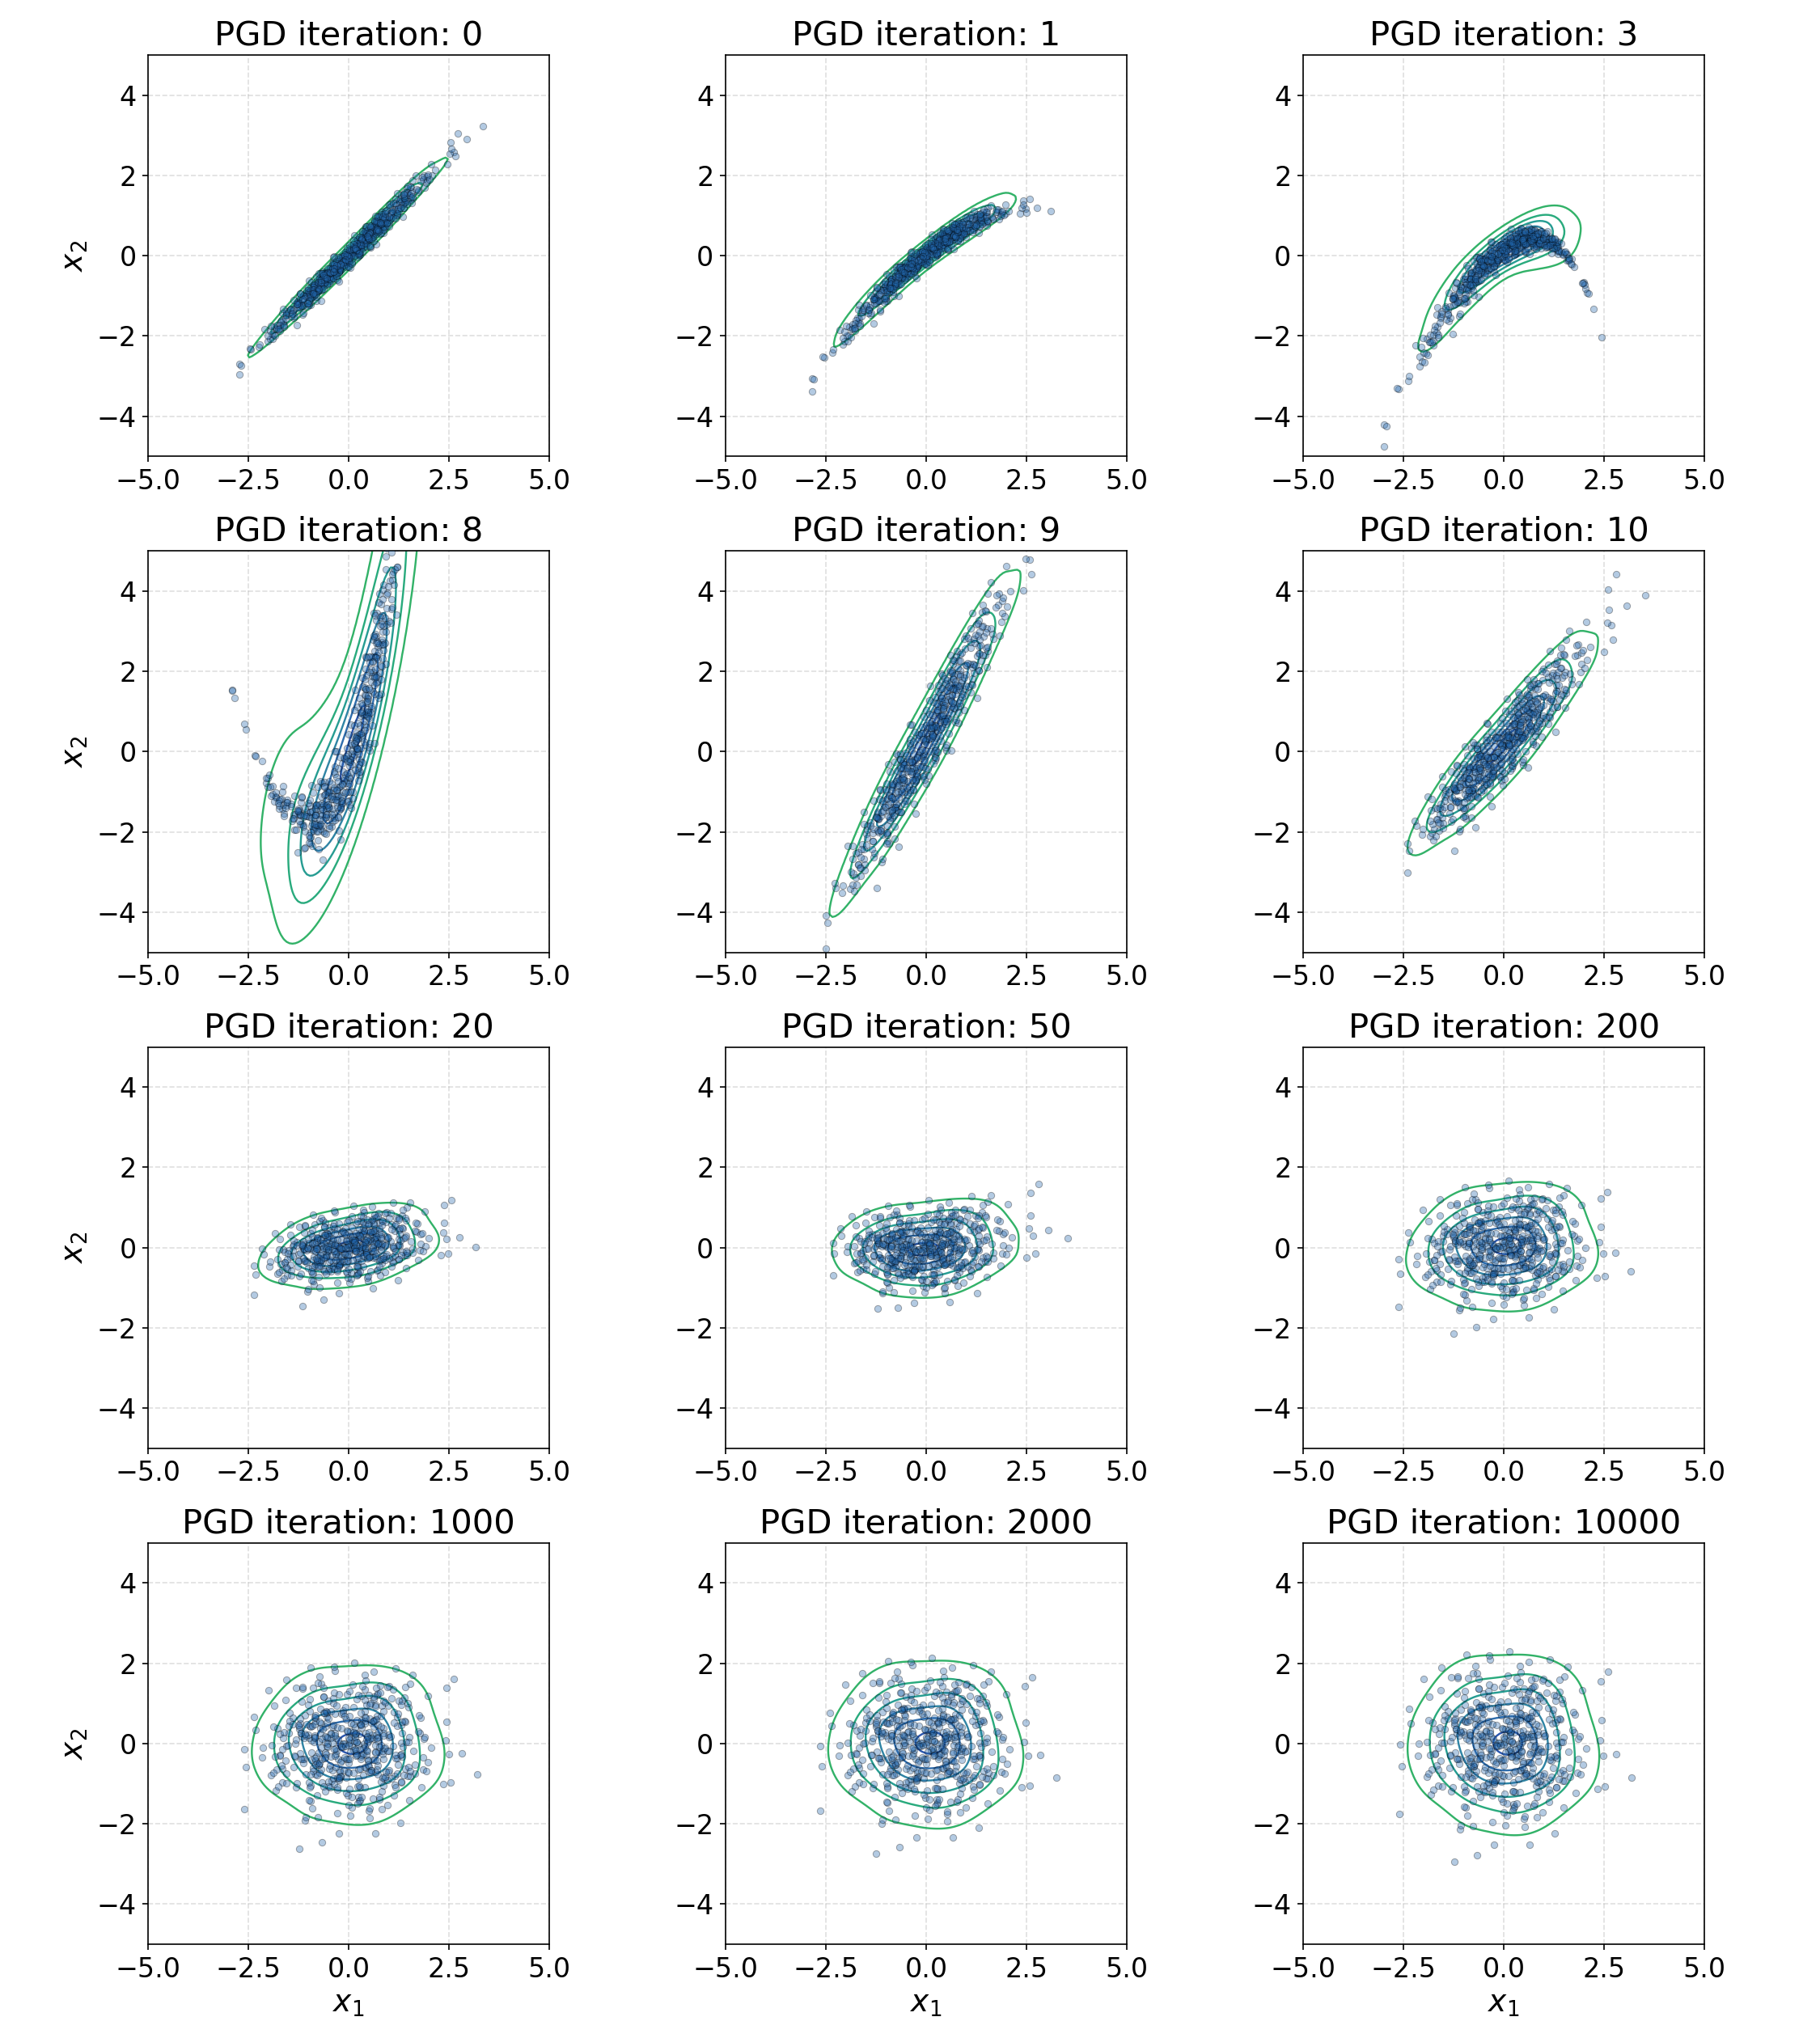
\includegraphics[width=\linewidth]{figures/line_shear_progress.png}
    \caption{Progress plot for the linear experiment (\texttt{SEED} $=2222$).}
    \label{fig:line_shear_progress}
\end{figure}

\begin{figure}[htbp]
    \centering
    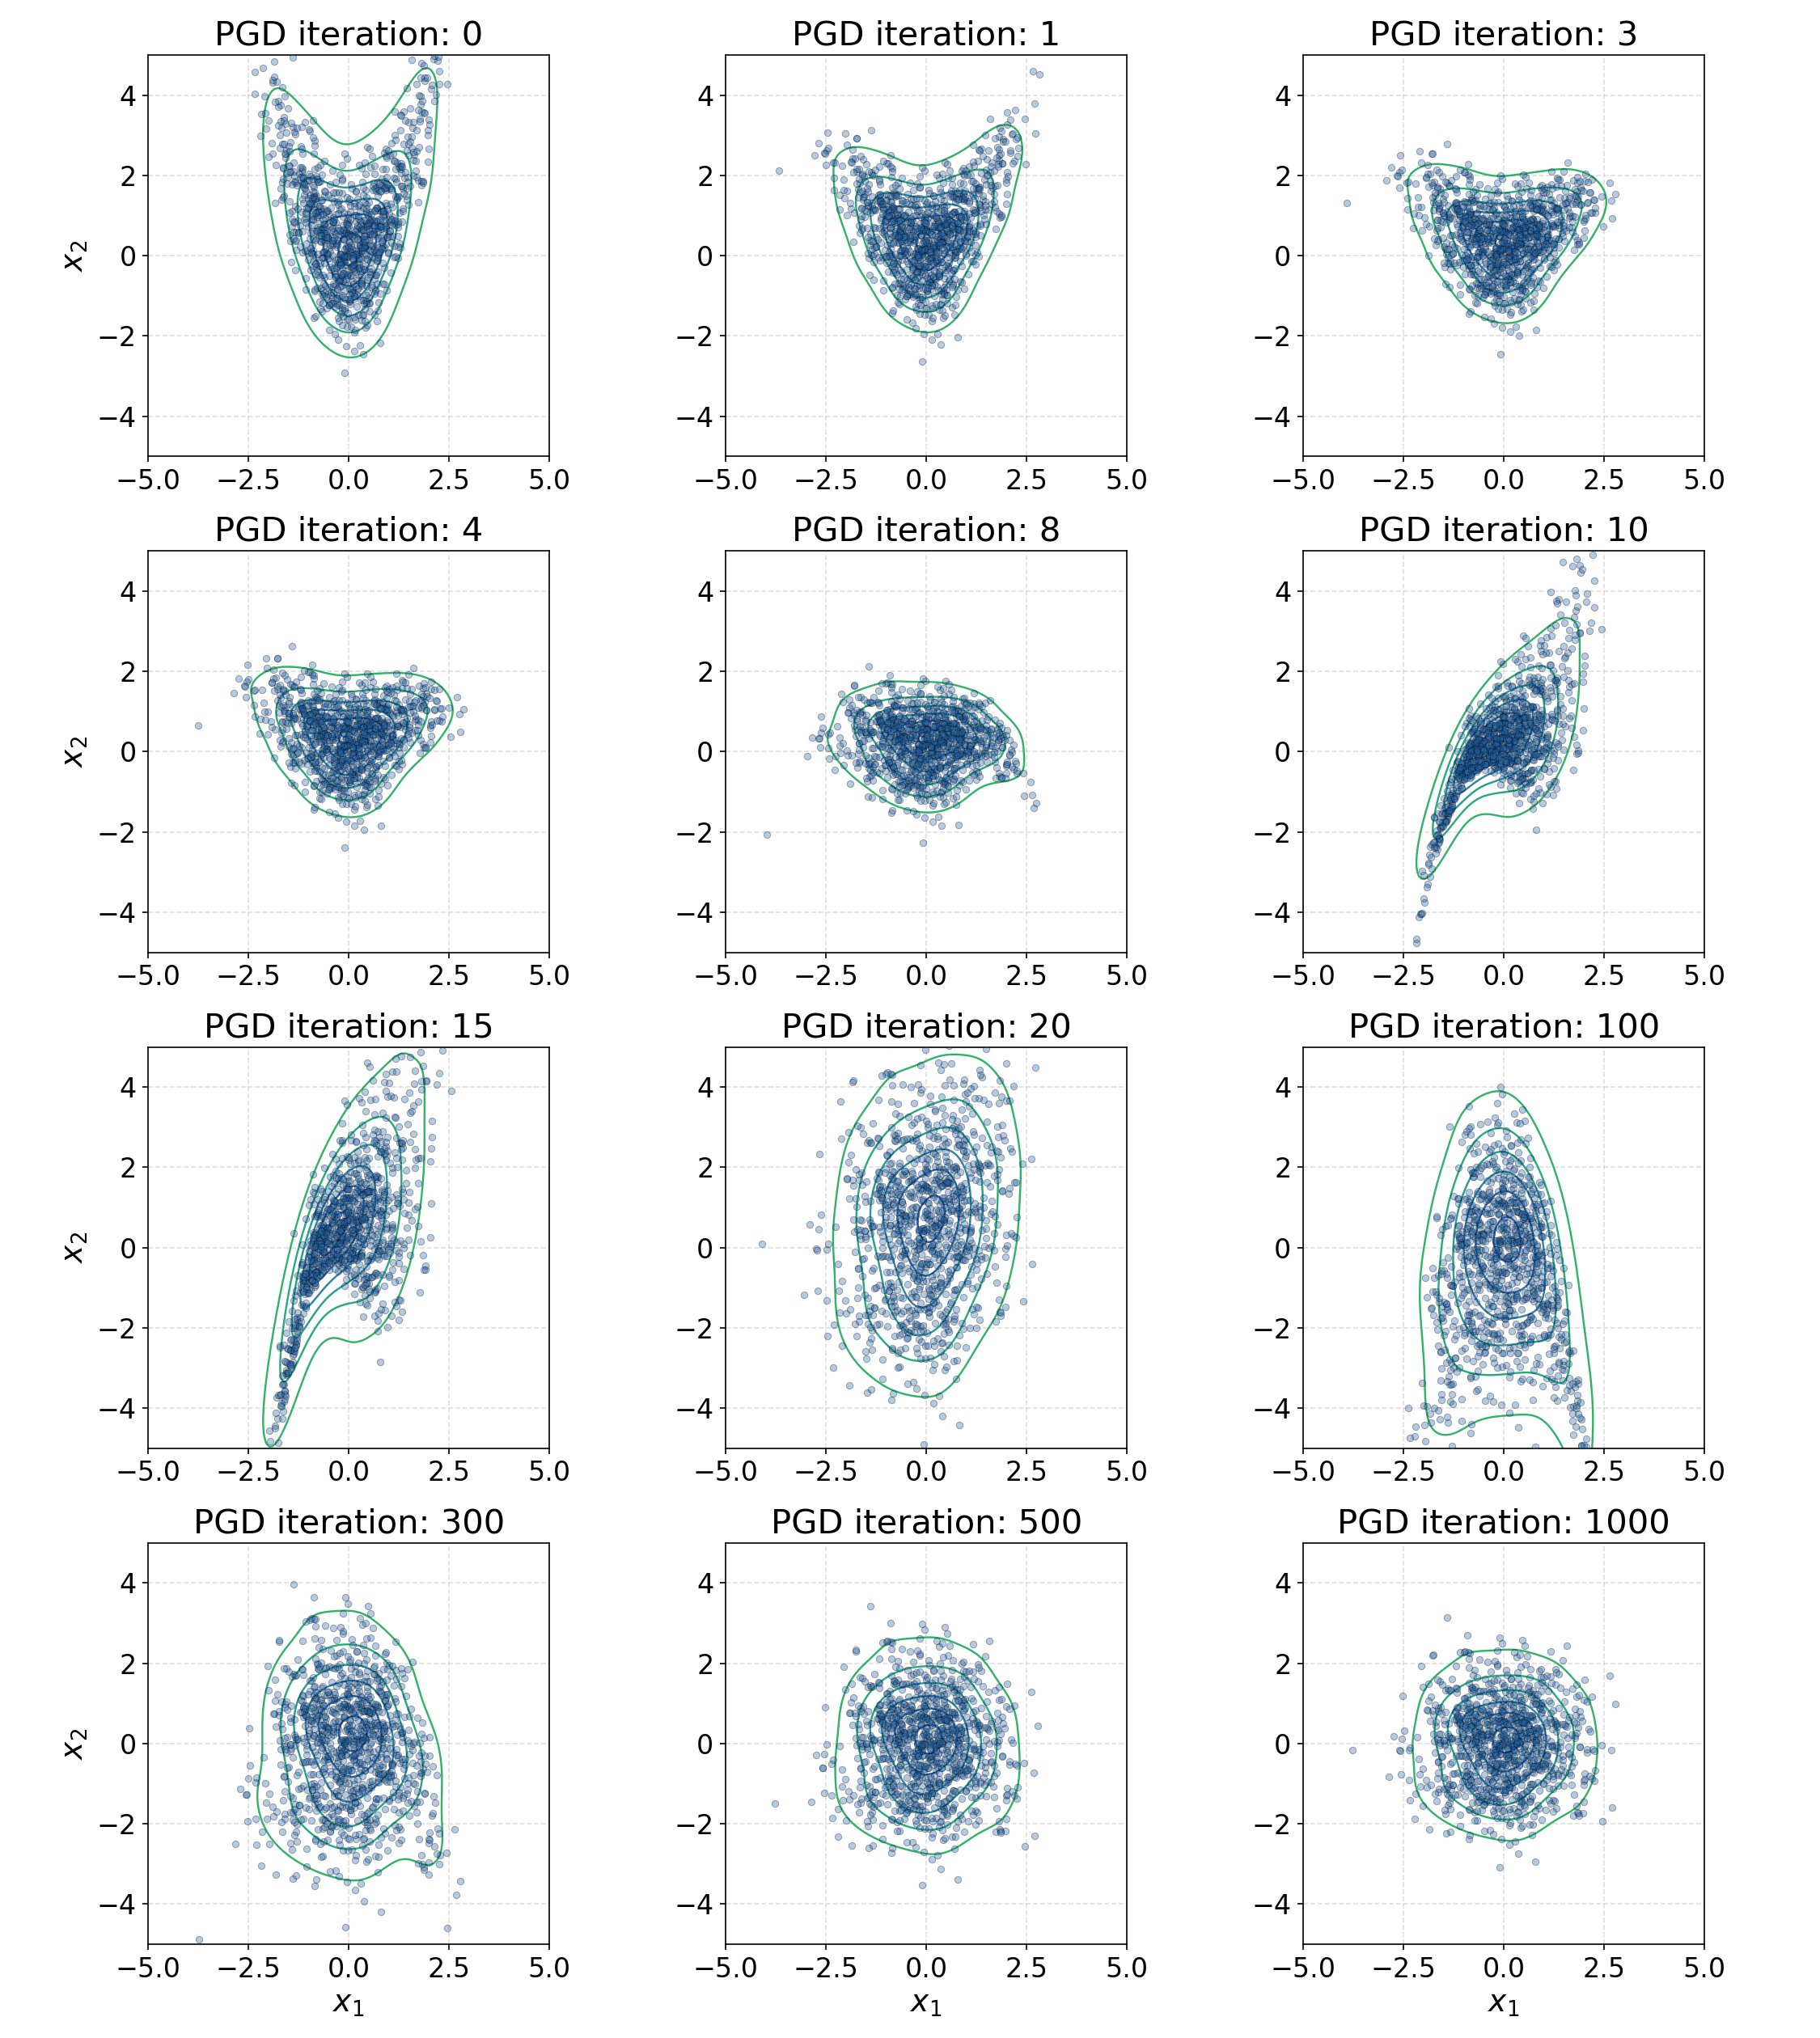
\includegraphics[width=\linewidth]{figures/quadratic_shear_progress.png}
    \caption{Progress plot for the quadratic experiment (\texttt{SEED} $=5432$).}
    \label{fig:quadratic_shear_progress}
\end{figure}

\begin{figure}[htbp]
    \centering
    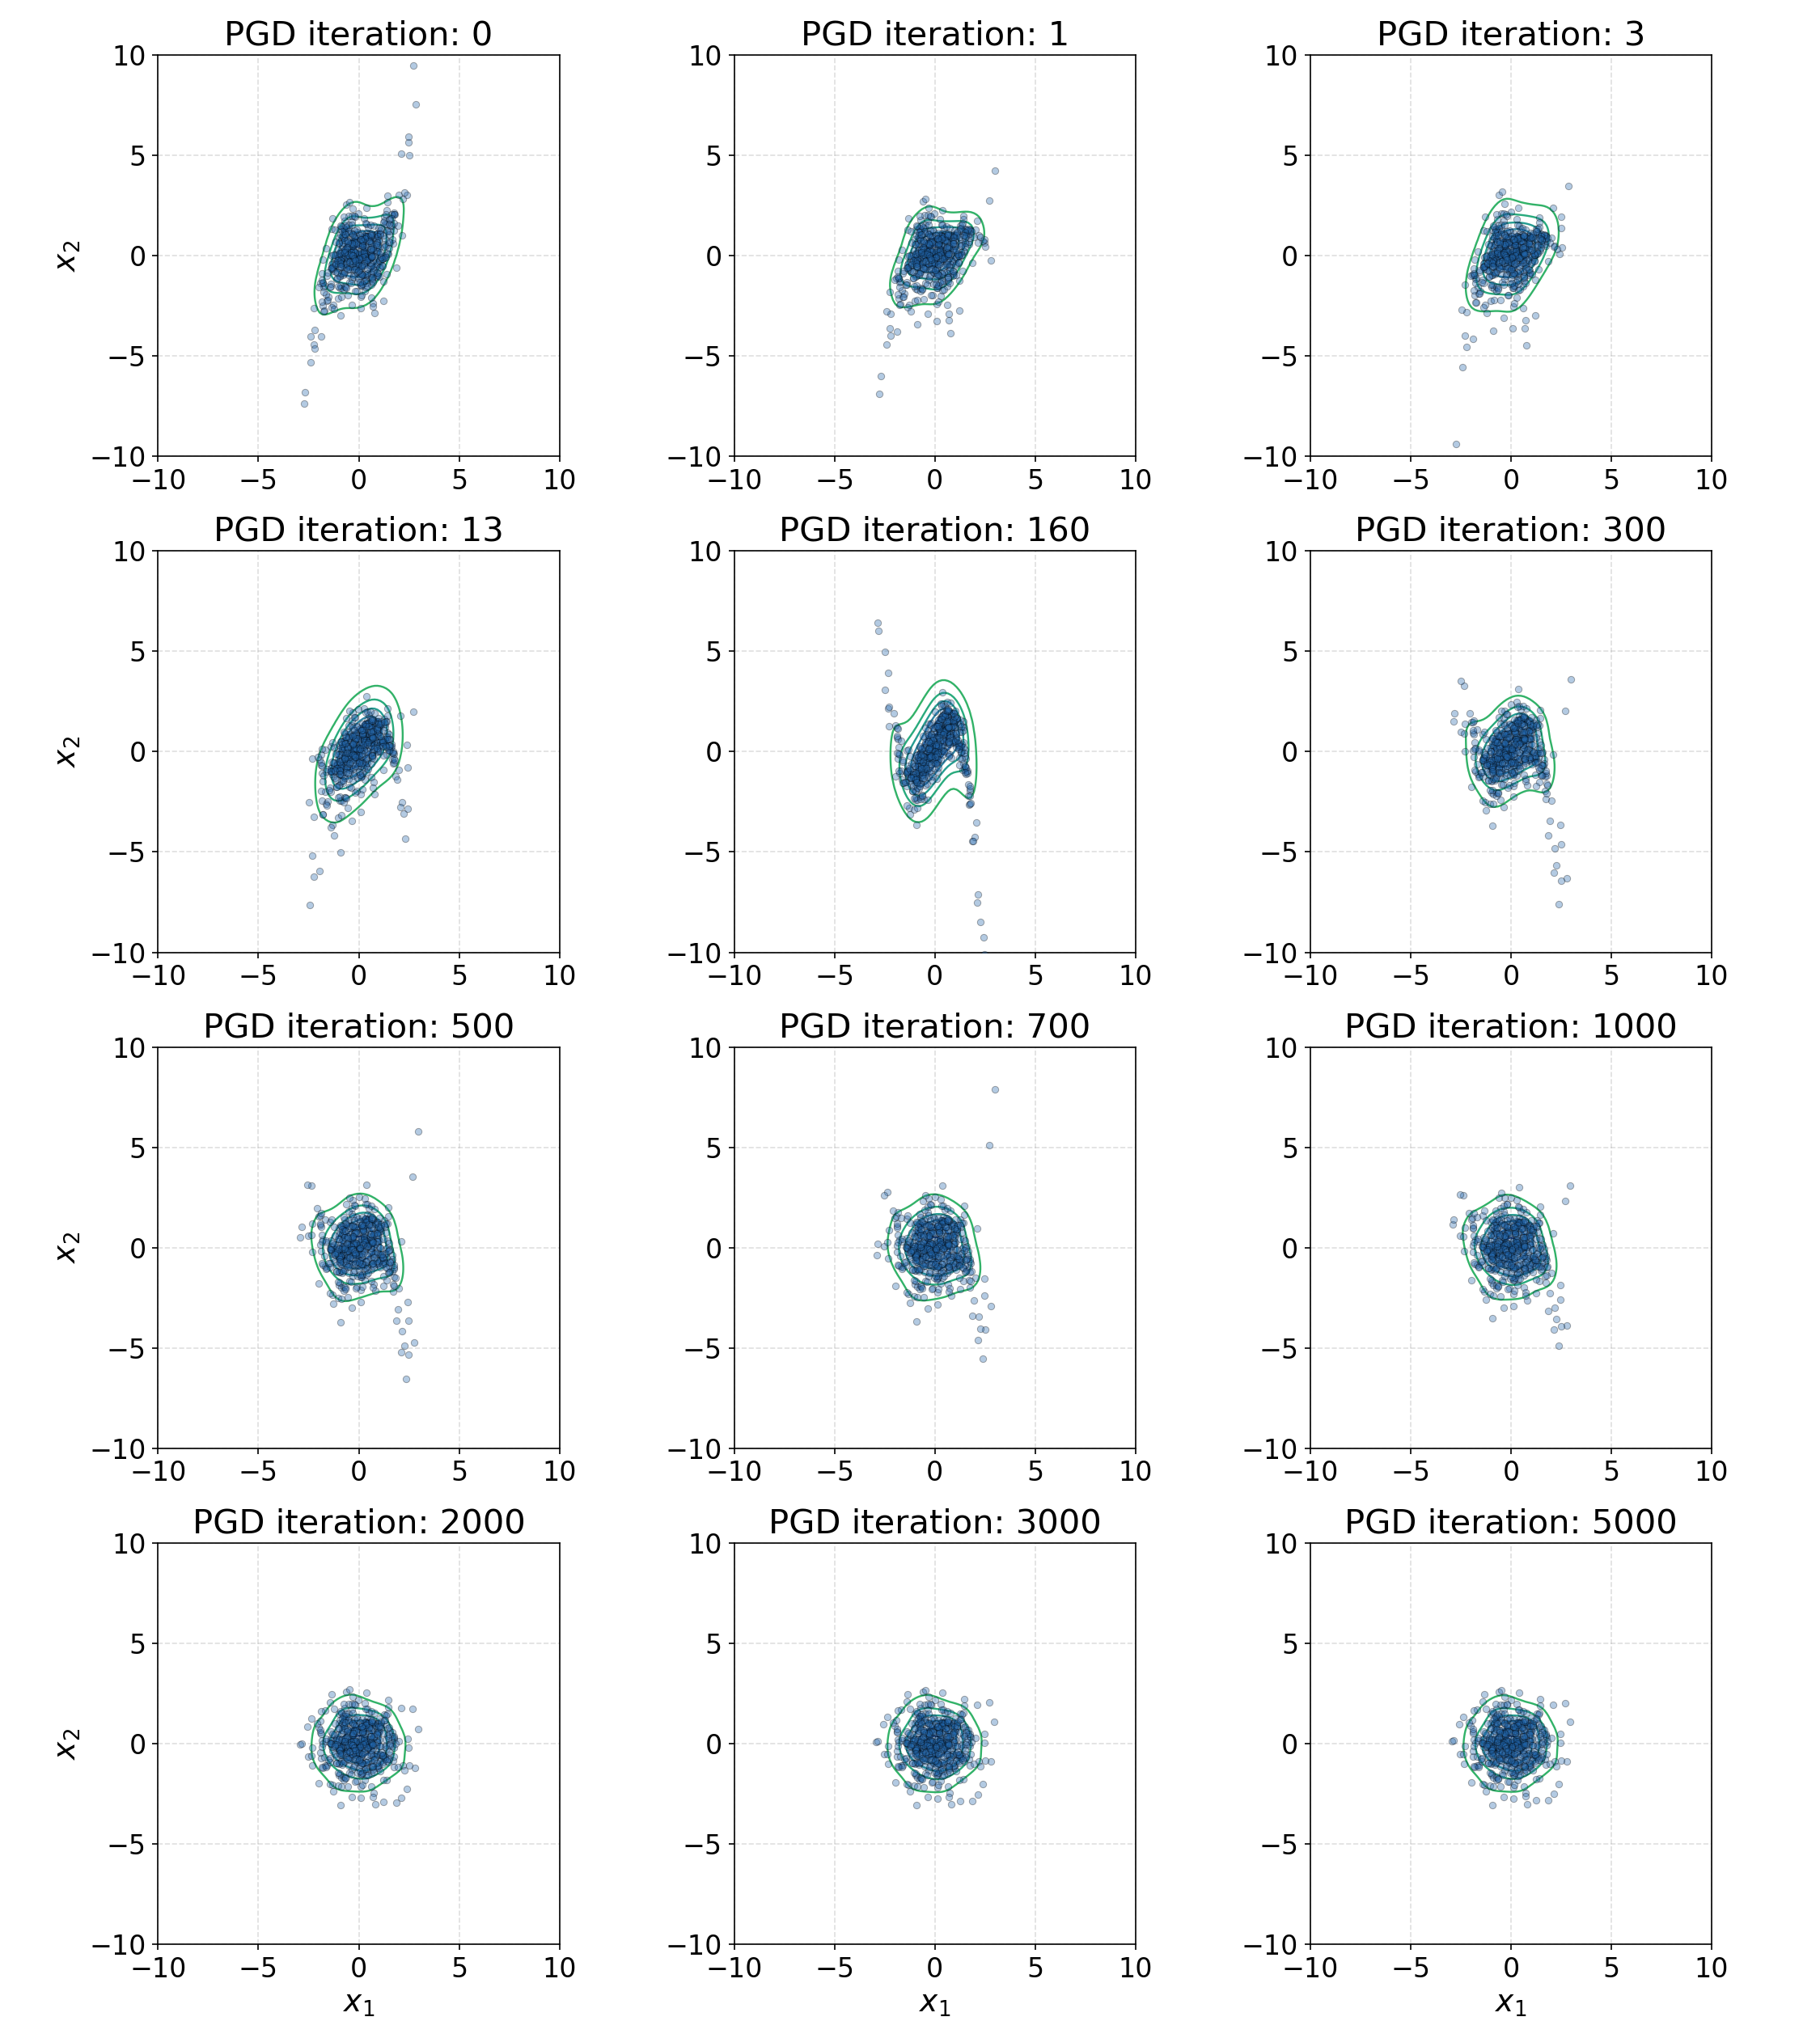
\includegraphics[width=\linewidth]{figures/cubic_shear_progress.png}
    \caption{Progress plot for the cubic experiment (\texttt{SEED} $=507$).}
    \label{fig:cubic_shear_progress}
\end{figure}


